\documentclass[conference]{IEEEtran}
\IEEEoverridecommandlockouts
\usepackage{graphicx} % Required for inserting images
\usepackage{mathtools}
\usepackage{amsfonts}
\usepackage{subfig}
\usepackage{caption}
\usepackage{amsmath}
\usepackage{xcolor}


\title{Traffic State-Based Adaptive Cruise Control}

% \author{\IEEEauthorblockN{Daechul Jung}
% \IEEEauthorblockA{\textit{Department of Computer Science} \\
% \textit{Vanderbilt University}\\
% Nashville, TN, USA \\
% daechul.jung@vanderbilt.edu}
% \and
% \IEEEauthorblockN{Quang Pham}
% \IEEEauthorblockA{\textit{Department of Computer Science} \\
% \textit{Vanderbilt University}\\
% Nashville, TN, USA \\
% quang.m.pham@vanderbilt.edu}
% \and
% \IEEEauthorblockN{Kate Sanborn}
% \IEEEauthorblockA{\textit{Department of Computer Science} \\
% \textit{Vanderbilt University}\\
% Nashville, TN, USA \\
% kate.l.sanborn@vanderbilt.edu}
% \and
% \IEEEauthorblockN{Dan Work}
% \IEEEauthorblockA{\textit{Department of Civil and Environmental Engineering} \\
% \textit{Vanderbilt University}\\
% Nashville, TN, USA \\
% dan.work@vanderbilt.edu}
% \and
% \IEEEauthorblockN{Jonathan Sprinkle}
% \IEEEauthorblockA{\textit{Department of Computer Science} \\
% \textit{Vanderbilt University}\\
% Nashville, TN, USA \\
% jonathan.sprinkle@vanderbilt.edu}
% }

\author{
\IEEEauthorblockN{
Kate Sanborn\IEEEauthorrefmark{1},
Quang Pham\IEEEauthorrefmark{1},
Daechul Jung\IEEEauthorrefmark{1},
Dan Work\IEEEauthorrefmark{1},
Jonathan Sprinkle\IEEEauthorrefmark{1}
}

\IEEEauthorblockA{
\IEEEauthorrefmark{1}Department of Computer Science, Vanderbilt University\\
Nashville, TN 37235, USA\\
jonathan.sprinkle@vanderbilt.edu
}
}




\begin{document}

\maketitle

\begin{abstract}
Stop-and-go (phantom) traffic waves can be amplified by conventional adaptive cruise control (ACC) that reacts only to the immediate leader. We propose a traffic-wave phase–aware ACC that uses only onboard car-following signals (ego speed, gap, relative speed) to classify whether the ego vehicle is outside a wave, entering, inside, or exiting a stop-and-go wave, and then switches control parameters to damp disturbances while maintaining safety. In 25-vehicle simulations across 15 synthetic leader scenarios, increasing penetration of the proposed controller yields monotonic string-stability improvement and reduces peak acceleration transients (e.g., maximum jerk decreases from ~15 to ~6.8 m/s³ at full penetration). We further evaluate mixed-penetration platoons using NGSIM leader trajectories, showing reduced disturbance amplification in fleet speed distributions, but also identifying jerk increases at higher penetration due to abrupt mode transitions. These results motivate transition-smoothing as future work to preserve wave damping while improving comfort. Conclusions and future work for this project are also discussed.
\end{abstract}


\section{Introduction}

% {\color{blue} Add your group members, also and Jonathan and Dan, bring in better analysis of string stability, and provide lots of simulation results with real data to drive behavior.}

Standard Adaptive Cruise Control (ACC) systems typically only react to the immediate vehicle ahead but lack awareness of the larger traffic context. This could lead to amplification of phantom traffic jams, leading to string-unstable conditions, causing hard-braking events, stop-and-go waves and higher probability of rear-end collisions. In this paper, a “traffic wave” refers to a stop-and-go (phantom-jam) phenomenon that propagates upstream as a moving transition between higher-speed and lower-speed traffic, characterized locally by a sustained low-speed region and distinct entry/exit phases experienced by individual drivers.

This project addresses the limitation of reactive ACC by developing a Traffic State-Based ACC. Our system aims to do the following:

\begin{itemize}

\item Classify local traffic state: Use only onboard sensor data (velocity, space gap, relative velocity) to identify if the vehicle is in free-flow traffic, entering a traffic wave, inside a wave, or exiting a wave.
\item Proactively respond: Dynamically adapt the control strategy based on the classified state to ensure string stability, dampen wave propagation, and improve traffic flow efficiency.
\item Improve passenger comfort: Mitigate hard-braking events and send smoother control actions.
\end{itemize}

(This is newly added, needs review) This paper proposes a traffic state–based adaptive cruise control (ACC) strategy that mitigates stop-and-go traffic waves using only onboard car-following measurements. Our main contributions are: (1) a lightweight, real-time wave-phase classifier that labels the ego vehicle as outside, entering, inside, or exiting a stop-and-go wave based solely on ego speed, gap, and relative speed; (2) a mode-dependent ACC law that schedules control parameters across these phases to reduce disturbance amplification while maintaining safety constraints; and (3) a mixed-traffic evaluation using both synthetic leader scenarios and NGSIM-based leader trajectories, including penetration-rate sweeps and metrics for string stability and comfort (e.g., acceleration/jerk statistics) to quantify benefits and identify limitations due to mode switching.


\section{Related Works}
\subsection{Understanding the State of Traffic}
Stop-and-go waves can emerge unexpectedly even without bottlenecks, as presented experimentally by Sugiyama et al.\ \cite{Sugiyama2008}, this motivates real-time detection methods. Sakhare et al.\ \cite{futuretransp3040063} classify six shock-wave types from connected-vehicle GPS traces; Seo et al.\ \cite{7313231} use probe-vehicle spacing data and an Ensemble Kalman Filter to reconstruct density fields; and Cao et al.\ \cite{https://doi.org/10.1049/iet-its.2018.5124} detect end-of-queue shockwaves by combining local speed drops across multiple spacing-equipped probe vehicles. These methods share a common limitation: they require \emph{fleets} of instrumented or connected vehicles and, in some cases, offline post-processing. In contrast, our approach classifies the traffic wave phase using only onboard measurements from a \emph{single} ego vehicle in real time.

\subsection{ACC that Adapts to Traffic State}
Several ACC strategies have been implemented that dynamically adjust based on the state of traffic. Stern et al.\ \cite{STERN2018205} demonstrated that a single autonomous vehicle running the FollowerStopper controller can dampen stop-and-go waves on a ring road while reducing excessive braking and fuel consumption. Kesting et al.\ \cite{KESTING2008668} designed a traffic-state-adaptive ACC that detects five congestion phases and schedules IDM parameters accordingly; their system improved stability and capacity in simulation but relies on GPS-assisted bottleneck detection and a moving-average velocity classifier that introduces identification delay. Spiliopoulou et al.\ \cite{doi:10.1177/0361198118796020} and Elmorshedy et al.\ \cite{doi:10.1177/03611981231152459} both adjust ACC headway settings to maximize throughput, but depend on vehicle-to-infrastructure communication or roadside detectors for section-level flow and speed measurements.

An important motivation for traffic-state-adaptive control is the empirical finding that commercially deployed ACC systems are not string stable. Gunter et al.\ \cite{Gunter2021StringStable} tested production ACC vehicles and showed that they amplify velocity disturbances, contributing to stop-and-go wave formation rather than suppressing it. This underscores the need for controllers that actively account for the surrounding traffic state. On the theoretical side, Ploeg et al.\ \cite{Ploeg2014} formalize $\mathcal{L}_p$ string stability for cascaded vehicle-following systems and show that a constant time-headway policy can guarantee string stability under appropriate gain selection, providing the analytical foundation for the type of linear control law used in our work.

In the learning-enabled domain, Stojcsics et al.\ \cite{s21186089} pair a DNN classifier with an assurance monitor and predetermined safe strategies, illustrating how data-driven perception can be integrated without compromising control-layer safety guarantees.

Unlike the previous approaches, our controller requires neither GPS, V2I communication, nor multi-vehicle coordination. It uses a deterministic state machine operating on ego speed, gap, and relative speed to classify four wave phases in real time, and schedules mode-specific linear control gains to damp disturbances while maintaining safety constraints.

\section{Design}
Our design has two main components: classification and state-specific control. The goal of classification is to identify the state of overall traffic based on the behavior of the lead vehicle. The state then determines the control strategy that we use in the vehicle.

\subsection{Classification}

Our classification subsystem identifies four different modes of traffic.

\begin{enumerate}

    \item No wave: free flowing traffic or no lead vehicle present
    \item Into wave: vehicles are slowing down
    \item In wave: vehicles are moving slowly or stopped
    \item Out of wave: vehicles are accelerating out of a slow period
    
\end{enumerate}

We use a state machine to determine the state. Most of the transition criteria are determined based on the lead vehicle velocity and the lead vehicle acceleration. The state machine is shown in Figure \ref{fig:class_state}.


\begin{figure*}
    \centering
    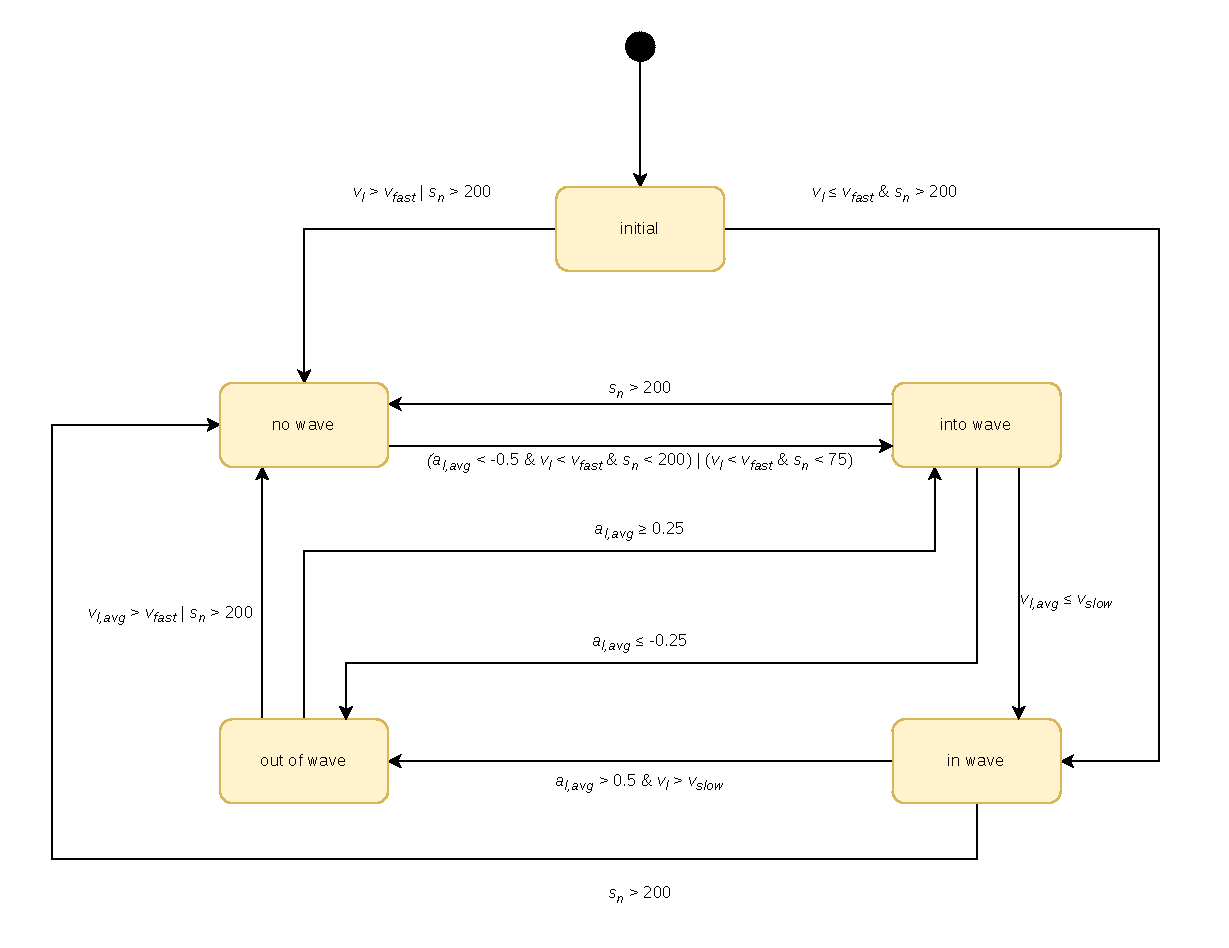
\includegraphics[width=0.7\linewidth]{figures/ITSC 2026 Group Project Classification.pdf}
    \caption{Classification state machine. $s_n$ is the space gap. $v_l$ is the lead vehicle velocity. $v_{l, avg}$ is the moving average of the lead vehicle velocity. $a_{l,avg}$ is the moving average of the lead vehicle acceleration. $v_{slow}$ (10 m/s) and $v_{fast}$ (13.5 m/s) are tunable transition thresholds.}
    \label{fig:class_state}
\end{figure*}

The initial state is determined by the lead vehicle velocity (ego velocity plus relative velocity). If the lead velocity is greater than the no wave velocity (set to 13.5 m/s, can be changed as a parameter) or the lead distance is greater than 200 meters, the initial state is set to no wave. Otherwise, the state is set to in wave.

The mode transitions from no wave to into wave if the lead vehicle is decelerating and the lead velocity is less than the no wave velocity.

There are three possible transitions out of the into wave mode. If the lead velocity decreases below the wave velocity (set to 10 m/s, can be changed as a parameter), the mode transitions to in wave. Another transition is to the out of wave mode. This transition is taken if the lead vehicle has a moving average acceleration greater than 0.25 m/s\textsuperscript{2}. The last transition is to the no wave mode. If the lead distance is greater than 200 meters (when the lead car disappears, for instance), the mode switches to no wave.

The in wave mode has two transitions. If the lead acceleration moving average is greater than 0.5 m/s\textsuperscript{2} and the lead velocity is greater than the wave velocity, the mode transitions to out of wave. If the lead distance is greater than 200 meters, the mode switches to no wave.

The out of wave mode has two transitions. If the velocity is greater than the no wave velocity or if the lead distance is greater than 200 meters, the mode transitions to no wave. If the lead acceleration moving average is less than -0.25 m/s\textsuperscript{2}, the mode switches to into wave.


\subsection{State-Specific Control Strategies}

The command acceleration strategy is selected by the classification mode. The into wave, in wave, and out of wave modes share a common linear control law with state-specific parameters:

\begin{equation}
    \frac{dv_n(t)}{dt} = \alpha (s_n(t)-(\tau v_n(t) + s_{min})) + k \Delta v
\end{equation}

The parameters for each mode are shown in Table \ref{tab:mode_param}.

\begin{table}[htbp]
\caption{Mode parameters for control}
\begin{center}
\begin{tabular}{|c|c|c|c|c|}
\hline
Mode & $\alpha$ & $\tau$ & $s_{min}$ & $k$ \\
\hline
No Wave & 0.615 & 2.266 & 10 & 0.221 \\
\hline
Into Wave & 0.700 & 2.400 & 10 & 0.230 \\
\hline
In Wave & 0.646 & 2.253 & 10 & 0.213 \\
\hline
Out of Wave & 1.100 & 2.400 & 10 & 0.240 \\
\hline
\end{tabular}
\label{tab:mode_param}
\end{center}
\end{table}

The into wave mode parameters allow the controller to aggressively reduce the speed to match traffic. The in wave parameters are designed to maintain stable following with conservative gains. The out of wave mode parameters allow the vehicle to rapidly accelerate away from slow traffic.

\subsubsection{No Wave Mode: Dynamic Velocity Limiting}

The no wave mode uses the same distance-based control law but adds a dynamic velocity-limiting layer. First, a safe velocity is computed from the kinematic stopping distance equation:

\begin{equation}
    v_{safe} = v_{lead} + \sqrt{2 \left| a_{max,decel} \right| \cdot \max(0,\; e_{gap})}
\end{equation}

where $e_{gap} = s_n - s_{min} - \tau \cdot v_n$ is the gap error and $a_{max,decel} = -3.0$~m/s$^2$ is the maximum deceleration. The effective desired velocity is then:

\begin{equation}
    v_{des} = \min(v_{max},\; v_{safe})
\end{equation}

A soft velocity limiter attenuates the distance-based acceleration as the ego velocity approaches the desired velocity:

\begin{equation}
    \lambda = \min\!\left(1,\; \frac{1}{3}\,\text{sat}(v_{des} - v_n,\, -6,\, 3)\right)
\end{equation}

The final commanded acceleration is:

\begin{equation}
    a_{cmd} = \min(\lambda \cdot a_{dist},\; a_{dist})
\end{equation}

where $a_{dist}$ is the saturated output of the linear control law. The $\min$ operator ensures that braking commands always pass through at full magnitude regardless of $\lambda$, while positive acceleration is smoothly attenuated as the vehicle approaches $v_{des}$. This prevents the vehicle from exceeding $v_{max}$ in free-flow conditions and ensures safe approach speeds when the gap error is small.

\section{Metrics for Success}

The three metrics that we wanted to test for our controller performance were smooth acceleration and deceleration, limiting hard braking, and string stability.

We evaluated three different simulations based on these metrics: a ROS and Docker simulation, a large-scale simulation using synthetic trajectories, and a large-scale simulation using trajectories from NGSIM \cite{FHWA_NGSIM_2006} data. The ROS and Docker simulation simulates a single vehicle following a recorded trajectory from real vehicle data. The large-scale simulation using synthetic trajectories simulates a fleet of 25 vehicles. The lead vehicle has synthetic behavior, such as a constant speed, hard brake, or oscillation. Different penetration rates of the experimental controller and the intelligent driver model (IDM) \cite{PhysRevE.62.1805} are tested. The large-scale NGSIM simulation also simulates a fleet of 25 vehicles. In this simulation, the lead vehicle trajectory comes from recorded vehicle behavior in the NGSIM dataset. Different penetration rates of the experimental controller and the IDM are tested. The following section describes the metrics and how they were analyzed in each of the simulations.

\subsection{Smoother Acceleration and Deceleration}

For smooth acceleration and deceleration, we decided to evaluate jerk. We wanted the derivative of acceleration to remain in a comfortable range.

\begin{equation}
    \left| \frac{da(t)}{dt} \right| < 0.5 m/s^3 
\end{equation}

% {\color{red} We evaluated the performance in terms of jerk for the multivehicle Simulink simulations and the large-scale simulations. The multivehicle Simulink simulations print a warning for every time step where this constraint is violated. In the large-scale simulations, the jerk is also calculated.}


In the ROS/Docker simulation, we compute jerk from the ego commanded-acceleration and evaluate the fraction of time \(\left| \frac{da(t)}{dt} \right|\) exceeds the comfort threshold \(0.5~\mathrm{m/s^3}\).


For the large-scale synthetic simulations, we compute the maximum jerk magnitude observed across all follower vehicles and evaluate whether it remains within a comfortable range. We also assess the mean jerk across the fleet at each penetration rate to determine whether higher ACC penetration reduces abrupt acceleration changes overall.

For the large-scale NGSIM simulations, we evaluate the average percentage of follower vehicle time spent experiencing high jerk events across different penetration rates of the experimental controller.

\subsection{Limit Hard Braking Events}

To evaluate the hard braking, we checked the amount of time with a command acceleration of -3.0 m/s\textsuperscript{2}. 
% {\color{red}In the multivehicle simulations, a warning is printed for every time step where this is violated. For the ROS/Docker simulations, the in-vehicle test, and the large-scale simulations, we graph all the command acceleration values over time and qualitatively evaluate the amount of time with the minimum acceleration value.}
In the ROS/Docker simulation, we utilize the command acceleration, we quantify and evaluate hard braking as the percentage of samples where \(a_{\mathrm{cmd}} \le -3.0~\mathrm{m/s^2}\).

For the large-scale synthetic simulations, we evaluate the maximum deceleration experienced by any follower vehicle across all scenarios and penetration rates. The hard braking threshold is $-3.0~\mathrm{m/s^2}$. We also monitor the minimum space gap to confirm that safety margins are maintained and no collision-risk events occur.

To evaluate hard braking in the NGSIM simulations, we evaluate the average percentage of follower vehicle time spent experiencing large deceleration across different penetration rates of the experimental controller.

\subsection{String Stability}

Another goal for this controller was not to magnify disturbances through a platoon of vehicles. 
% {\color{red} We mainly evaluated our performance on this metric through the large-scale simulations. In the synthetic data tests, we simulate a line of 25 vehicles where the first vehicle has behavior specified by a function. For these, we calculate string stability as the ratio of velocity variance of all the cars at the end of the simulation (last 20\%) versus the beginning of the simulation (first 20\%). The other large-scale simulations follow an NGSIM trajectory. For these simulations, we graph the velocity distributions from the beginning of the line of cars to the end and evaluate whether the range of velocity values increases or decreases.}

In ROS/Docker simulation, we evaluate string stability by comparing disturbance magnitudes such as \(\sigma(v_{\mathrm{ego}})/\sigma(v_{\mathrm{lead}})\) and calculating the relative speed \(v_{\mathrm{ego}}-v_{\mathrm{lead}}\) to confirm disturbances are not amplified.

For the large-scale synthetic simulations, we compute string stability as the ratio of velocity standard deviation of vehicles at the tail of the fleet to the velocity standard deviation of the lead vehicle. A ratio greater than one indicates amplification of disturbances (string instability), while a ratio less than one indicates dampening. We evaluate this metric across all 15 scenarios at each penetration rate.

In the NGSIM simulations, we plot the distribution of velocities of all the vehicles in the fleet to determine if large variations propagate backwards.

\section{Results}

\subsection{ROS and Docker Simulation}
The following section discusses the ROS/Docker simulation results for the three success metrics: smooth acceleration/deceleration (jerk), limiting hard braking, and string stability. Figure~\ref{fig:ros-jerk} shows the jerk time history computed from the commanded acceleration, and Figure~\ref{fig:ros-jerk-dist} shows the distribution of \(|j|\). The jerk remains near zero for most of the run, indicating generally smooth control actions, but exhibits brief threshold violations during an initial transient and a later adjustment interval. These transient spikes create a long-tailed \(|j|\) distribution and suggest that comfort can be improved by reducing abrupt changes during controller engagement and large corrections.

\begin{figure}
    \centering
    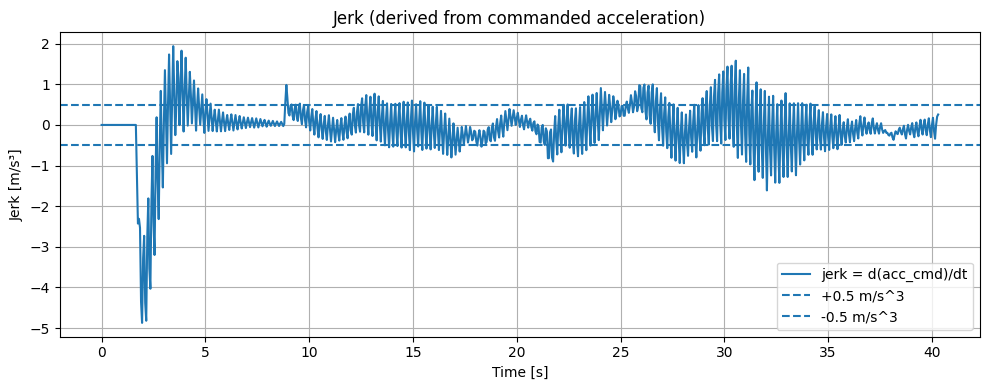
\includegraphics[width=\linewidth]{figures/jerk_distribution.png}
    \caption{ROS/Docker simulation jerk results: time history and \(|j|\) distribution.}
    \label{fig:ros-jerk}
\end{figure}
\begin{figure}
    \centering
    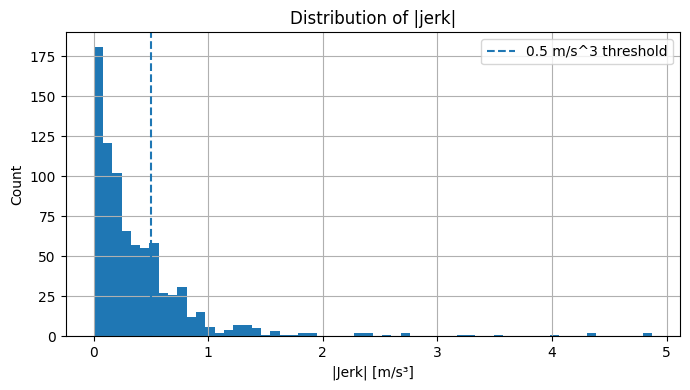
\includegraphics[width=\linewidth]{figures/jerk_distribution2.png}
    \caption{ROS/Docker simulation jerk distribution: histogram of \(|j|\) distribution.}
    \label{fig:ros-jerk-dist}
\end{figure}
Figure~\ref{fig:ros-hard-brake} shows the commanded acceleration \(a_{\mathrm{cmd}}\) over time with the hard-braking threshold marked. Across the entire ROS/Docker run, the commanded acceleration stays well above the hard-braking region, indicating that the controller avoids harsh deceleration and remains in a moderate braking regime. Overall, the ROS/Docker results demonstrate that the controller satisfies the hard-braking safety objective in this single-lead/single-follower scenario.

\begin{figure}
    \centering
    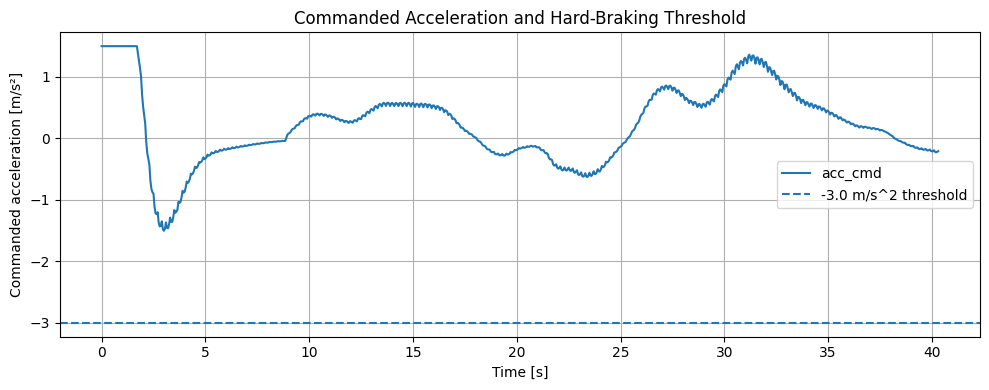
\includegraphics[width=\linewidth]{figures/limit_hard_breaking.png}
    \caption{ROS/Docker simulation commanded acceleration with hard-braking threshold.}
    \label{fig:ros-hard-brake}
\end{figure}

To evaluate string stability in the ROS/Docker setting, which contains a single lead--ego pair rather than a full platoon, we use a single-follower based on the propagation of speed disturbances from the lead vehicle to the ego vehicle. Figure~\ref{fig:ros-string} compares the lead and ego velocity traces and summarizes the relative speed behavior. The ego vehicle does not exhibit larger oscillations than the lead vehicle, and speed disturbances are not amplified in the follower, indicating stable tracking without sustained growth in oscillations. Under this proxy metric, the ROS/Docker results are consistent with string-stable behavior for the tested scenario.

\begin{figure}
    \centering
    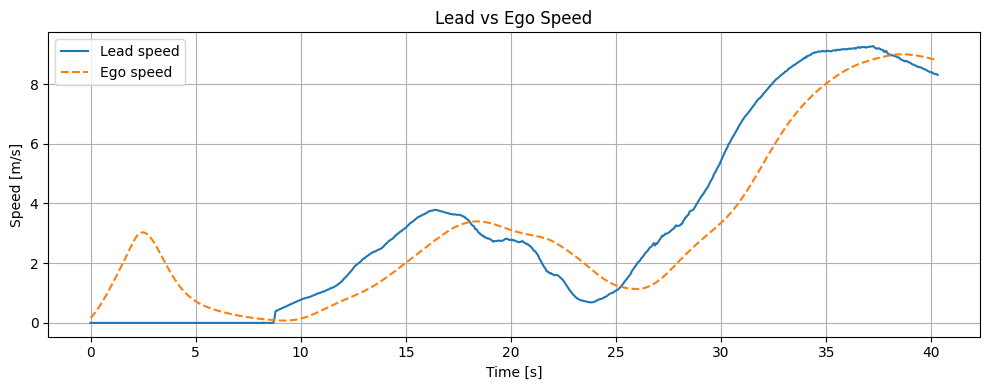
\includegraphics[width=\linewidth]{figures/string_stability.png}
    \caption{ROS/Docker simulation string-stability results using lead and ego velocity signals.}
    \label{fig:ros-string}
\end{figure}


\subsection{Synthetic Trajectory Simulation}

We evaluated the controller in a large-scale fleet simulation with 25 vehicles, a 100-second duration, and a 0.05-second time step. The lead vehicle follows synthetic trajectories across 15 scenarios in five categories: constant speed (15, 20, 25~m/s), oscillation (small, medium, large amplitude, multi-frequency), sudden acceleration (gradual, rapid), sudden deceleration (gradual, rapid, severe), and step changes (two-state, three-state, frequent). Penetration rates of 5\%, 10\%, 20\%, 50\%, 75\%, and 100\% were tested at each scenario. Vehicles not running the experimental controller use the IDM.

Table~\ref{tab:synth-summary} summarizes string stability improvement and minimum space gap across the five scenario categories. String stability is computed as the ratio of tail-vehicle to lead-vehicle velocity standard deviation; values below 1.0 indicate disturbance attenuation.

\begin{table}[htbp]
\caption{Synthetic simulation results: string stability ratio and minimum space gap at 5\% vs.\ 100\% ACC penetration.}
\begin{center}
\begin{tabular}{|l|c|c|c|}
\hline
\textbf{Category} & \textbf{SS (5\%$\to$100\%)} & \textbf{Improv.} & \textbf{Min Gap (5\%$\to$100\%)} \\
\hline
Constant speed & 2.7$\to$0.0 & $\sim$100\% & 29--57$\to$43--68~m \\
\hline
Oscillation$^*$ & 2.1--3.6$\to$0.4--2.1 & 41--82\% & 40--44$\to$45--50~m \\
\hline
Accel.\ transient & 0.5--0.6$\to$0.1 & 86--88\% & 29$\to$43~m \\
\hline
Decel.\ transient & 20--48$\to$0.4--2.6 & 98--99\% & 18--29$\to$33--43~m \\
\hline
Step changes$^*$ & 0.3--2.1$\to$0.2--0.8 & 13--90\% & 31--42$\to$43--50~m \\
\hline
\end{tabular}
\label{tab:synth-summary}
\end{center}
\vspace{-0.5em}
{\footnotesize $^*$Excludes multi-frequency oscillation (02d), where string stability degraded from 1.86 to 10.8 at 100\% penetration; see text.}
\end{table}

The controller's largest impact is on sudden-deceleration scenarios — the most safety-critical category — where string stability ratios collapse from 20--48$\times$ (severe amplification under IDM-dominated fleets) to 0.4--2.6 at full penetration, and minimum gaps increase from 18~m to 33~m. Constant-speed following achieves near-perfect attenuation (ratio $\to$ 0), and single-frequency oscillation scenarios show 41--82\% improvement, with the controller acting as a wave absorber. Figure~\ref{fig:synth-decel-comparison} illustrates the penetration-rate dependence for the rapid deceleration scenario (25$\to$15~m/s in 2~s).

\begin{figure}
    \centering
    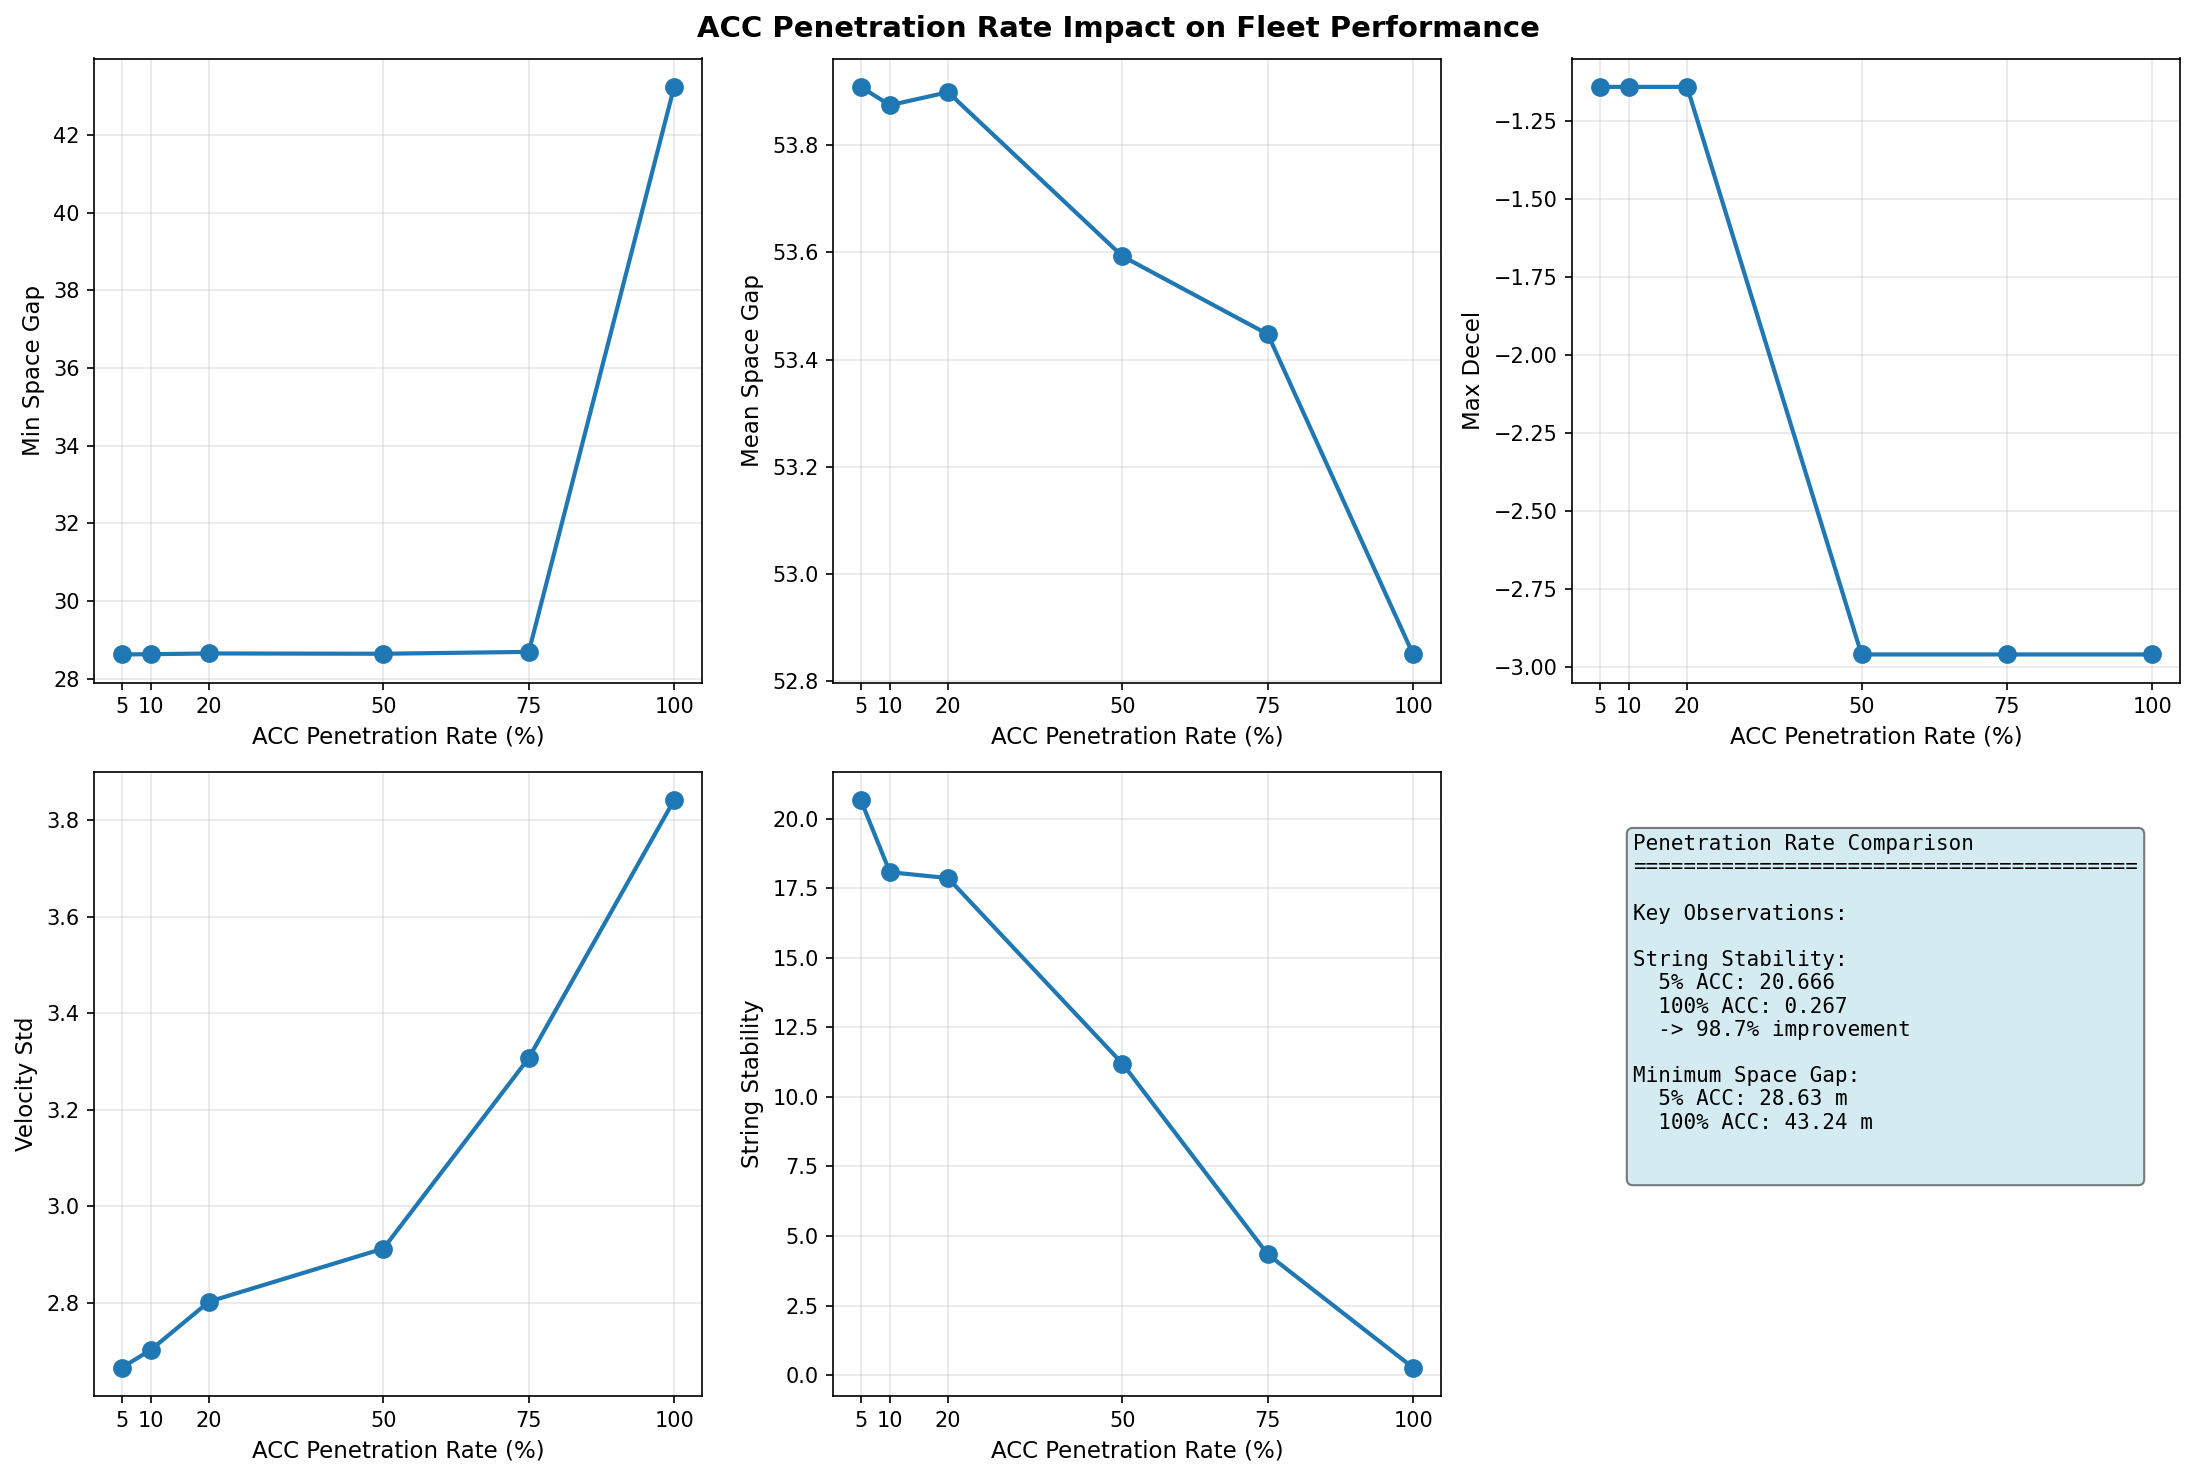
\includegraphics[width=\linewidth]{figures/synth_04b_sudden_decel_rapid_comparison.png}
    \caption{Rapid deceleration scenario: fleet metrics vs.\ ACC penetration rate.}
    \label{fig:synth-decel-comparison}
\end{figure}

Two failure modes were identified. In the multi-frequency oscillation scenario (superimposed 40~s and 10~s periods), string stability degraded from 1.86 at 5\% to 10.8 at 100\% penetration, indicating that the state machine's transition logic interacts poorly with complex wave spectra. In the two-state step-change scenario (15$\leftrightarrow$25~m/s every 15~s), the string stability ratio increased from 0.33 to 0.83 — still below 1.0 (string-stable), but less effective than the IDM fleet. Minimum space gaps nonetheless improved in both cases, so safety was not compromised.

Across all 15 scenarios, maximum jerk decreased from $\sim$15~m/s$^3$ at 5\% penetration to 6.8~m/s$^3$ at 100\%, as the IDM's abrupt reactions were replaced by smoother ACC commands. Maximum deceleration stayed within the $-3.0$~m/s$^2$ hard-braking limit for all scenarios except the severe stress test (25$\to$10~m/s in 3~s), and minimum space gaps increased monotonically with penetration rate across every scenario tested.

\subsection{NGSIM Trajectory Simulation}

The following section discusses the results of following an NGSIM trajectory with varying penetration rates of the experimental controller. Figure \ref{fig:ngsim-0-vel} shows the velocities of the fleet when all following vehicles use the IDM. Figure \ref{fig:ngsim-0-vel-dist} shows the distribution of the velocities of all vehicles. It is clear that by itself, the IDM propagates and amplifies disturbances backwards in the lane of vehicles. The traffic wave amplifies backwards. Even though the leader never comes to a full stop, several following vehicles are forced to stop.

\begin{figure}
    \centering
    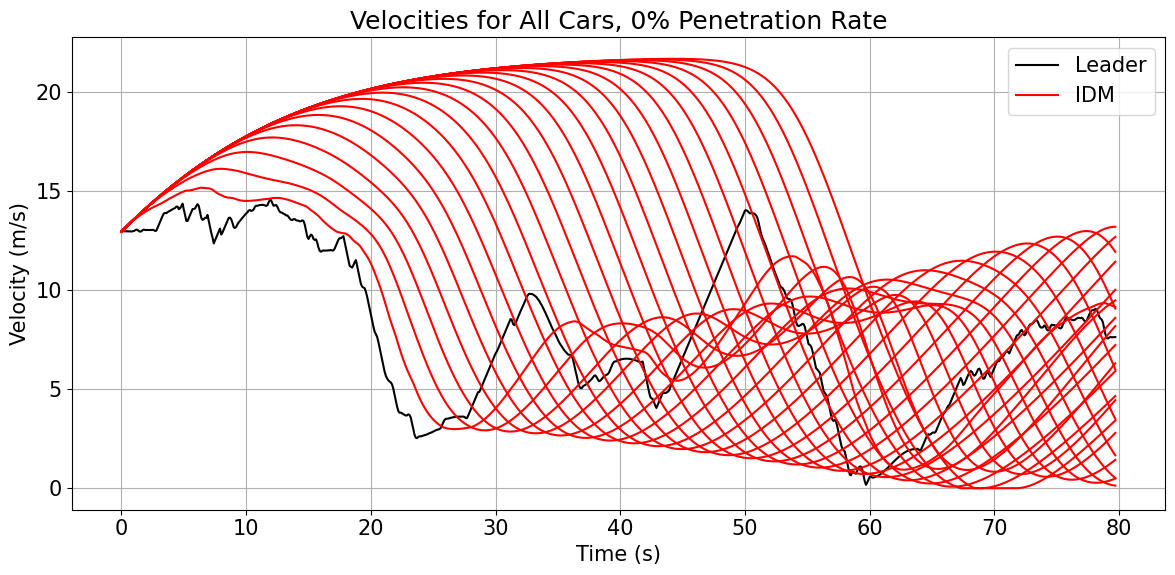
\includegraphics[width=\linewidth]{figures/ID 350 0 percent velocities.png}
    \caption{NGSIM simulation fleet velocities, 0\% penetration}
    \label{fig:ngsim-0-vel}
\end{figure}


\begin{figure}
    \centering
    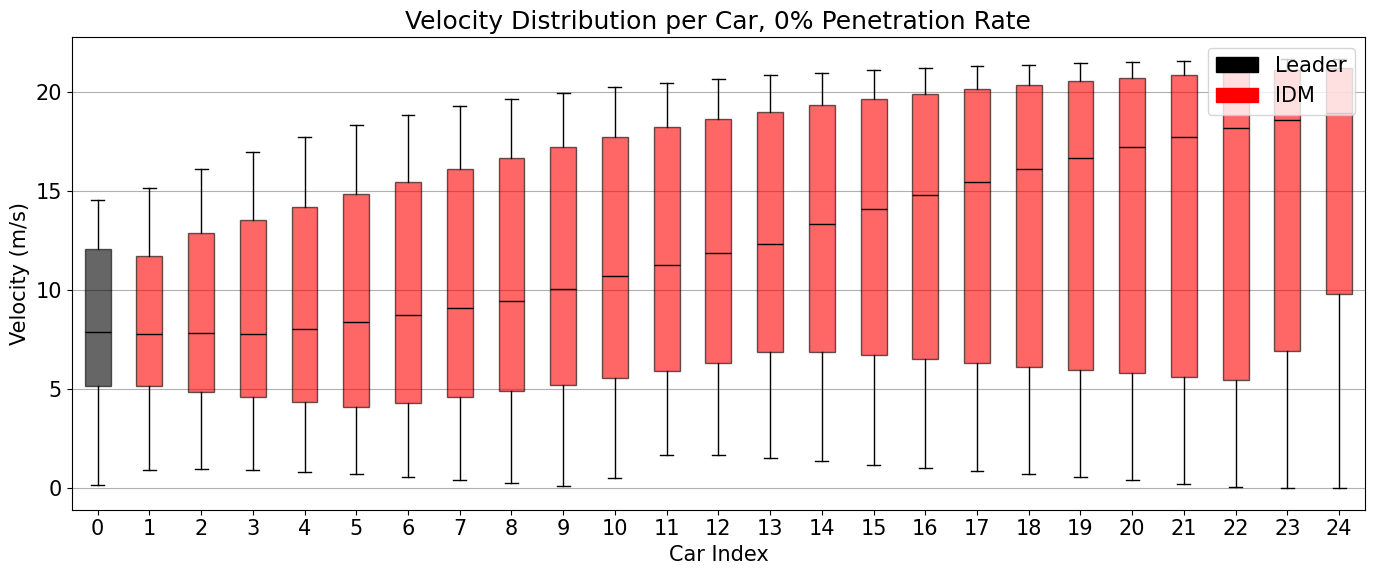
\includegraphics[width=\linewidth]{figures/ID 350 0 percent velocity distrbution.png}
    \caption{NGSIM simulation fleet velocity distributions, 0\% penetration}
    \label{fig:ngsim-0-vel-dist}
\end{figure}

Figure \ref{fig:ngsim-50-vel} shows the velocities of the fleet when half of the following vehicles use the IDM and the rest run the experimental controller. Figure \ref{fig:ngsim-50-vel-dist} shows the distribution of the velocities of all vehicles. While the disturbance is still propagated some in the fleet, the amplification is less. The range of velocities of the experimental controller is typically less than the range of the velocities of the preceding vehicle. None of the vehicles are forced to halt entirely.

\begin{figure}
    \centering
    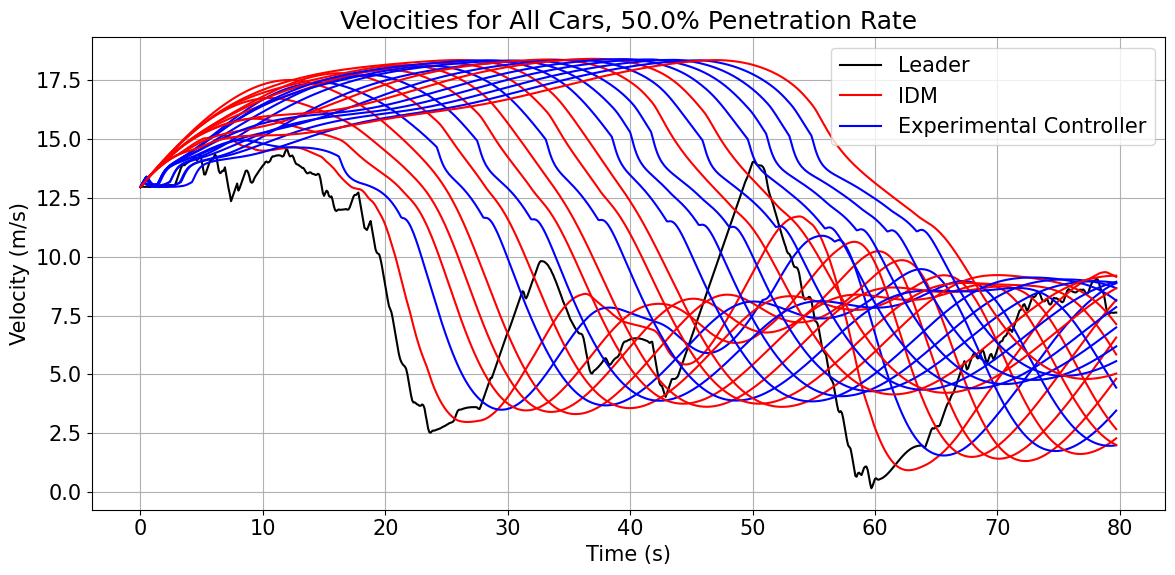
\includegraphics[width=\linewidth]{figures/ID 350 50 percent velocities.png}
    \caption{NGSIM simulation fleet velocities, 50\% penetration}
    \label{fig:ngsim-50-vel}
\end{figure}

\begin{figure}
    \centering
    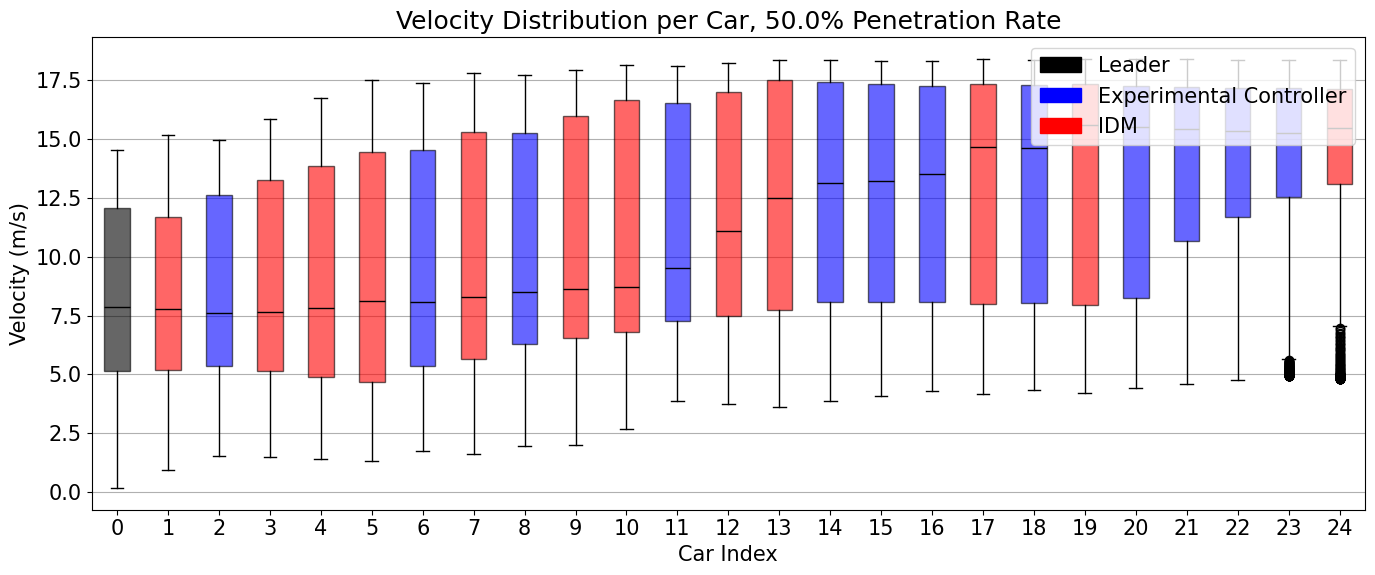
\includegraphics[width=\linewidth]{figures/ID 350 50 percent velocity distrbution.png}
    \caption{NGSIM simulation fleet velocity distributions, 50\% penetration}
    \label{fig:ngsim-50-vel-dist}
\end{figure}

Figure \ref{fig:ngsim-100-vel} shows the velocities of the fleet when all vehicles use the experimental controller. Figure \ref{fig:ngsim-100-vel-dist} shows the distribution of the velocities of all vehicles. Disturbances are dampened. Also, the velocity distribution shrinks backwards in the line of vehicles.


\begin{figure}
    \centering
    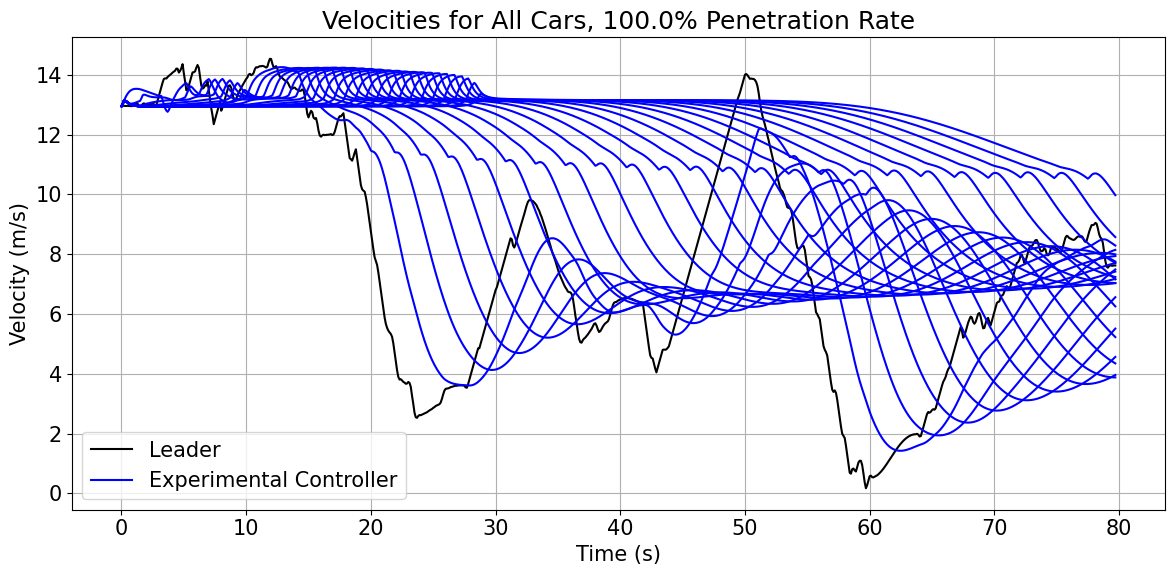
\includegraphics[width=\linewidth]{figures/ID 350 100 percent velocities.png}
    \caption{NGSIM simulation fleet velocities, 100\% penetration}
    \label{fig:ngsim-100-vel}
\end{figure}

\begin{figure}
    \centering
    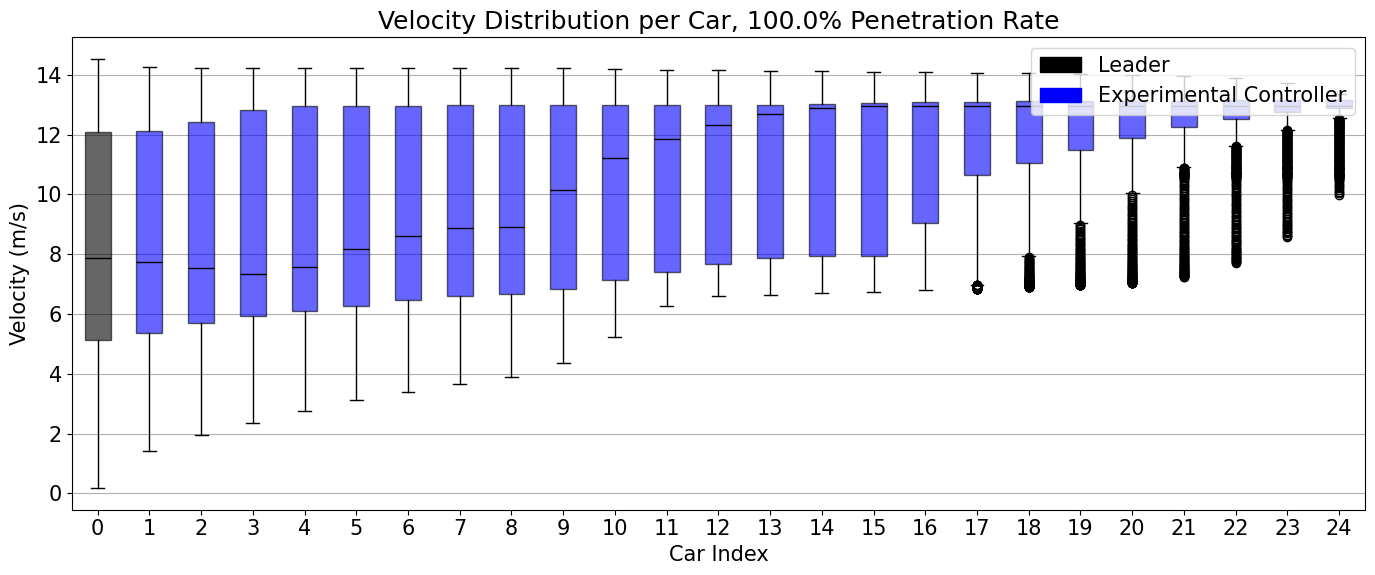
\includegraphics[width=\linewidth]{figures/ID 350 100 percent velocity distrbution.png}
    \caption{NGSIM simulation fleet velocity distributions, 100\% penetration}
    \label{fig:ngsim-100-vel-dist}
\end{figure}

In Figure \ref{fig:ngsim-jerk}, the average time that follower vehicles experience high jerk is shown. Overall, high jerk events increase as the penetration rate increases.

\begin{figure}
    \centering
    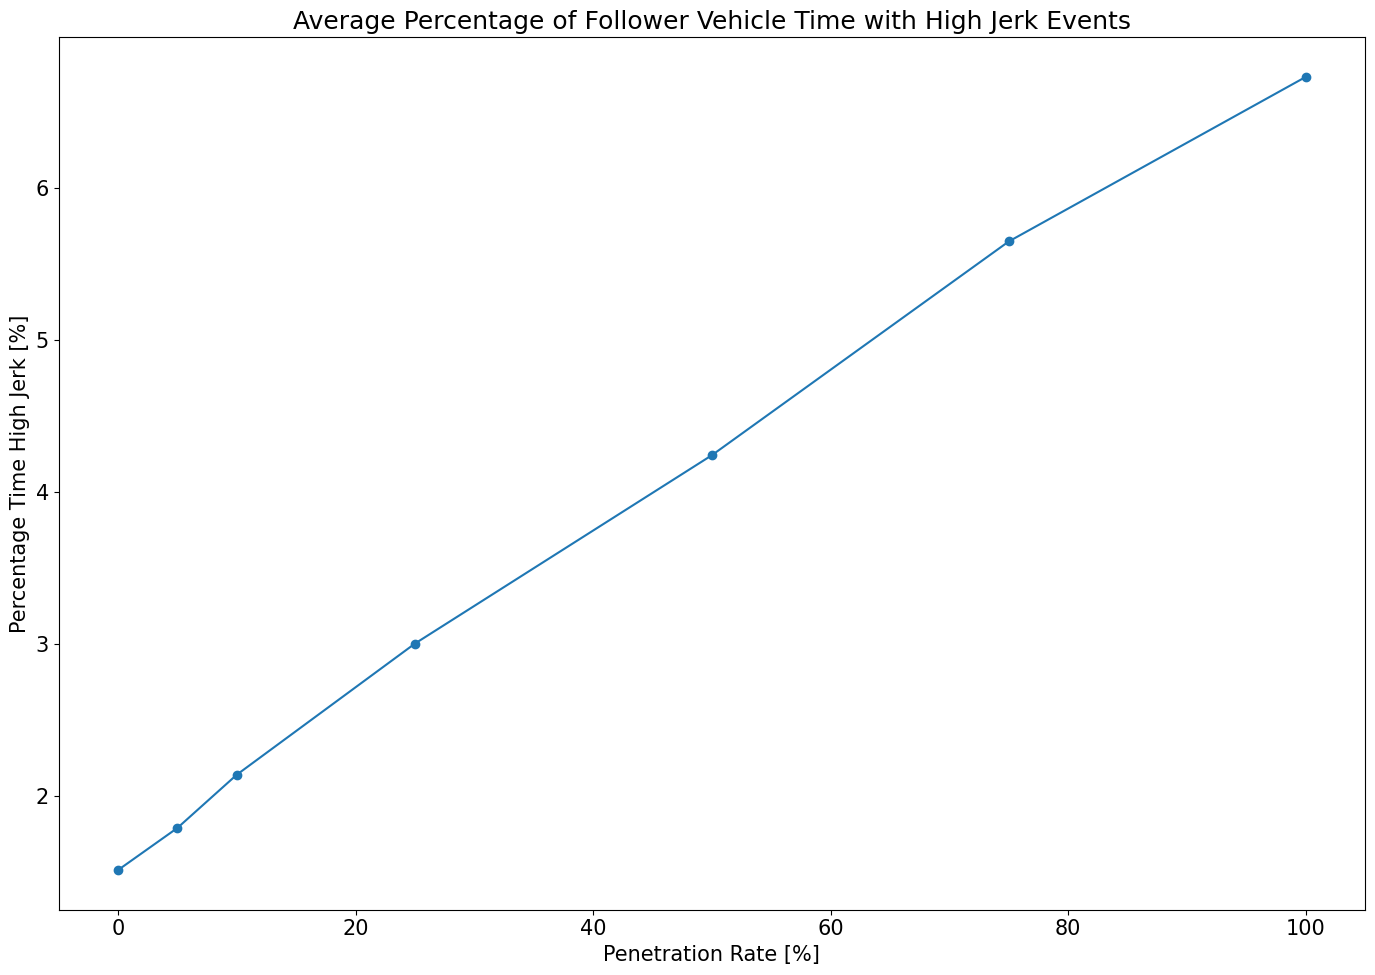
\includegraphics[width=0.75\linewidth]{figures/ID 350 large jerk.png}
    \caption{NGSIM simulation jerk events at varying penetration rates}
    \label{fig:ngsim-jerk}
\end{figure}

Across all penetration rates, the amount of time hard braking was constant. With only the IDM, no hard braking was required, and the hard braking did not increase as the penetration increased.

% \begin{figure}
%     \centering
%     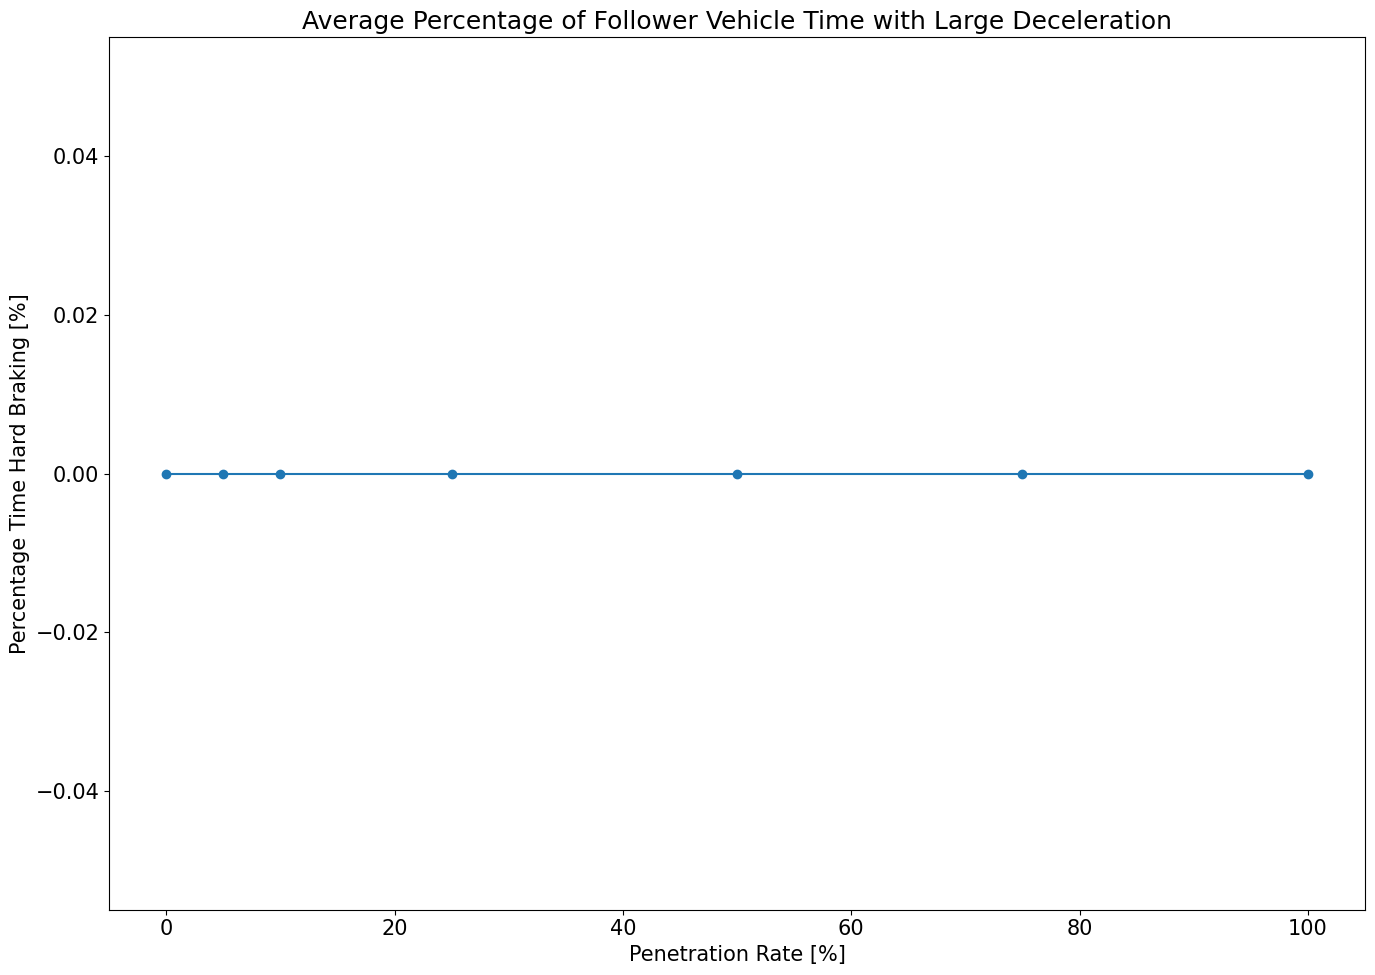
\includegraphics[width=0.75\linewidth]{figures/ID 350 large brake.png}
%     \caption{NGSIM simulation hard braking events at varying penetration rates}
%     \label{fig:ngsim-large-brake}
% \end{figure}

\section{Conclusions}

\subsection{Evaluation of Metrics}

\subsubsection{Smoother Acceleration and Deceleration}

The jerk signal remained small for much of the run, but showed clear threshold violations during transient periods, indicating that smooth acceleration/deceleration was not consistently maintained; therefore, this success metric was not fully achieved.

In the large-scale synthetic simulations, maximum jerk decreased from approximately 15~m/s$^3$ at 5\% penetration to 6.8~m/s$^3$ at 100\% penetration, as human driver reactions were replaced by smoother ACC commands. This metric was achieved for the synthetic simulations.

In the NGSIM simulations, high jerk increased with increasing penetration rates, likely due to abrupt acceleration changes at mode switches. This goal was not accomplished.

\subsubsection{Limit Hard Braking Events}

The commanded acceleration never entered the hard-braking region over the recorded run, demonstrating that the controller avoided harsh deceleration; this success metric was achieved.


In the large-scale synthetic simulations, the maximum deceleration stayed above the $-3.0$~m/s$^2$ hard braking threshold across all scenarios except the severe deceleration stress test (25 to 10~m/s in 3~seconds), which reached $-3.0$~m/s$^2$ by design. Minimum space gaps remained well above the 5~m safety threshold in all cases and increased with penetration rate. This metric was achieved.

The NGSIM simulations showed that adding the number of vehicles running the experimental controller did not increase hard braking. This metric was achieved.

\subsubsection{String Stability}

Using a single-follower proxy, the ego vehicle did not amplify lead-vehicle speed disturbances and the relative speed error stayed bounded, suggesting stable following behavior, hence the success metric was achieved.

In the large-scale synthetic simulations, string stability improved monotonically with penetration rate across all 15 scenarios. Constant-speed scenarios achieved up to 100\% improvement, oscillation scenarios achieved 41--82\% improvement, and even the most challenging step-change scenarios showed consistent gains. This metric was achieved.

In the distribution plots for the NGSIM, it is clear that the experimental controller avoids amplifying disturbances, showing that the new controller is string stable. The goal of string stability was accomplished.

\subsection{Future Work}

 For future work, the control parameters can be tuned to reduce jerk. The main source of jerk is likely abrupt mode switching, so smoothing the transition may eliminate these rapid changes in acceleration.
 It may also be beneficial to tune parameters across all modes using machine learning techniques. Using data-driven approaches to optimize across the three metrics may improve performance and help improve overall traffic flow.

\bibliographystyle{ieeetr}
\bibliography{References}

\end{document}
